\documentclass[a4paper,11pt]{article}
\usepackage[margin=20mm]{geometry}
\usepackage[T1]{fontenc}
\usepackage{lmodern,amsmath,amssymb,booktabs,graphicx,array}
\usepackage{microtype,xcolor,listings,hyperref}
\hypersetup{colorlinks=true,linkcolor=blue!45!black,urlcolor=blue!45!black,citecolor=blue!45!black}
\lstset{basicstyle=\ttfamily\small,breaklines=true,columns=fullflexible,frame=single,showstringspaces=false}
\setlength{\parskip}{0.25em}
\AtBeginDocument{%
  \setlength{\abovedisplayskip}{8pt plus 2pt minus 3pt}%
  \setlength{\belowdisplayskip}{8pt plus 2pt minus 3pt}%
}
\setlength{\textfloatsep}{12pt plus 2pt minus 2pt}
\setlength{\parindent}{0pt}
\makeatletter
\renewcommand\section{\@startsection{section}{1}{\z@}{-2.5ex plus -1ex minus -.2ex}{1.2ex plus .2ex}{\normalfont\Large\bfseries}}
\renewcommand\subsection{\@startsection{subsection}{2}{\z@}{-2ex plus -.7ex minus -.2ex}{.8ex plus .2ex}{\normalfont\large\bfseries}}
\makeatother
\newcommand{\code}[1]{\texttt{#1}}
% generated by scripts/analyze.py
\newcommand{\ScalingHistoricalStandardTwo}{1.96}
\newcommand{\ScalingHistoricalStandardFour}{3.84}
\newcommand{\ScalingHistoricalStandardEight}{6.91}
\newcommand{\ScalingHistoricalStandardSixteen}{8.82}
\newcommand{\ThroughputHistoricalStandardMax}{0.355}
\newcommand{\ScalingExtendedStandardTwo}{2.02}
\newcommand{\ScalingExtendedStandardFour}{4.06}
\newcommand{\ScalingExtendedStandardEight}{7.59}
\newcommand{\ScalingExtendedStandardSixteen}{13.10}
\newcommand{\ThroughputExtendedStandardMax}{11.660}
\newcommand{\ScalingHistoricalWideTwo}{1.96}
\newcommand{\ScalingHistoricalWideFour}{3.80}
\newcommand{\ScalingHistoricalWideEight}{7.37}
\newcommand{\ScalingHistoricalWideSixteen}{9.57}
\newcommand{\ThroughputHistoricalWideMax}{0.147}
\newcommand{\ScalingExtendedWideTwo}{2.02}
\newcommand{\ScalingExtendedWideFour}{4.06}
\newcommand{\ScalingExtendedWideEight}{8.08}
\newcommand{\ScalingExtendedWideSixteen}{13.48}
\newcommand{\ThroughputExtendedWideMax}{9.163}
\newcommand{\SpeedupWeeklyOptimized}{22.86}
\newcommand{\SpeedupWeeklyOptimizedLow}{21.61}
\newcommand{\SpeedupWeeklyOptimizedHigh}{24.14}
\newcommand{\SpeedupWeeklyExtended}{22.05}
\newcommand{\SpeedupWeeklyExtendedLow}{21.00}
\newcommand{\SpeedupWeeklyExtendedHigh}{23.10}
\newcommand{\SpeedupMonthlyOptimized}{10.01}
\newcommand{\SpeedupMonthlyOptimizedLow}{9.85}
\newcommand{\SpeedupMonthlyOptimizedHigh}{10.17}
\newcommand{\SpeedupMonthlyExtended}{21.31}
\newcommand{\SpeedupMonthlyExtendedLow}{20.99}
\newcommand{\SpeedupMonthlyExtendedHigh}{21.63}
\newcommand{\SpeedupIrregularOptimized}{2.65}
\newcommand{\SpeedupIrregularOptimizedLow}{2.55}
\newcommand{\SpeedupIrregularOptimizedHigh}{2.75}
\newcommand{\SpeedupIrregularExtended}{21.18}
\newcommand{\SpeedupIrregularExtendedLow}{20.98}
\newcommand{\SpeedupIrregularExtendedHigh}{21.39}
\newcommand{\GapRandomOverSorted}{3.06}
\newcommand{\GapRandomOverSortedLow}{3.04}
\newcommand{\GapRandomOverSortedHigh}{3.08}
\newcommand{\GapTableGainIrregular}{13.62}
\newcommand{\GapTableGainIrregularLow}{13.52}
\newcommand{\GapTableGainIrregularHigh}{13.74}
\newcommand{\GapDirectOverTableIrregular}{5.68}
\newcommand{\GapDirectOverTableIrregularLow}{5.57}
\newcommand{\GapDirectOverTableIrregularHigh}{5.79}
\newcommand{\KernelPowIncrYear}{17.07}
\newcommand{\KernelPowIncrYearLow}{16.67}
\newcommand{\KernelPowIncrYearHigh}{17.47}
\newcommand{\KernelAutodiffIncrYear}{120.80}
\newcommand{\KernelAutodiffIncrYearLow}{119.03}
\newcommand{\KernelAutodiffIncrYearHigh}{122.61}
\newcommand{\KernelPowIncrDecade}{19.95}
\newcommand{\KernelPowIncrDecadeLow}{19.59}
\newcommand{\KernelPowIncrDecadeHigh}{20.32}
\newcommand{\KernelAutodiffIncrDecade}{134.73}
\newcommand{\KernelAutodiffIncrDecadeLow}{128.77}
\newcommand{\KernelAutodiffIncrDecadeHigh}{141.17}
\newcommand{\PrepRatioDaily}{2.69}
\newcommand{\PrepRatioDailyLow}{2.57}
\newcommand{\PrepRatioDailyHigh}{2.82}
\newcommand{\PrepHistoricalTime}{9.974}
\newcommand{\PrepDigestTime}{3.706}
\newcommand{\SpeedupPreparedStandard}{23.53}
\newcommand{\SpeedupPreparedStandardLow}{22.80}
\newcommand{\SpeedupPreparedStandardHigh}{24.26}
\newcommand{\SpeedupPreparedStandardExtended}{23.76}
\newcommand{\SpeedupPreparedStandardExtendedLow}{23.08}
\newcommand{\SpeedupPreparedStandardExtendedHigh}{24.45}
\newcommand{\SpeedupPreparedWide}{48.28}
\newcommand{\SpeedupPreparedWideLow}{47.50}
\newcommand{\SpeedupPreparedWideHigh}{49.06}
\newcommand{\SpeedupPreparedWideExtended}{48.63}
\newcommand{\SpeedupPreparedWideExtendedLow}{47.87}
\newcommand{\SpeedupPreparedWideExtendedHigh}{49.39}
\newcommand{\SpeedupPreparedJcurve}{22.61}
\newcommand{\SpeedupPreparedJcurveLow}{22.30}
\newcommand{\SpeedupPreparedJcurveHigh}{22.92}
\newcommand{\SpeedupPreparedJcurveExtended}{23.13}
\newcommand{\SpeedupPreparedJcurveExtendedLow}{22.81}
\newcommand{\SpeedupPreparedJcurveExtendedHigh}{23.46}
\newcommand{\SpeedupPreparedSignflips}{34.65}
\newcommand{\SpeedupPreparedSignflipsLow}{33.58}
\newcommand{\SpeedupPreparedSignflipsHigh}{35.78}
\newcommand{\SpeedupPreparedSignflipsExtended}{39.01}
\newcommand{\SpeedupPreparedSignflipsExtendedLow}{38.14}
\newcommand{\SpeedupPreparedSignflipsExtendedHigh}{39.93}
\newcommand{\SpeedupDatedStandard}{6.83}
\newcommand{\SpeedupDatedStandardLow}{6.61}
\newcommand{\SpeedupDatedStandardHigh}{7.07}
\newcommand{\SpeedupDatedStandardExtended}{6.83}
\newcommand{\SpeedupDatedStandardExtendedLow}{6.58}
\newcommand{\SpeedupDatedStandardExtendedHigh}{7.09}
\newcommand{\SpeedupDatedWide}{14.41}
\newcommand{\SpeedupDatedWideLow}{14.16}
\newcommand{\SpeedupDatedWideHigh}{14.66}
\newcommand{\SpeedupDatedWideExtended}{13.68}
\newcommand{\SpeedupDatedWideExtendedLow}{13.50}
\newcommand{\SpeedupDatedWideExtendedHigh}{13.86}
\newcommand{\SpeedupDatedJcurve}{6.89}
\newcommand{\SpeedupDatedJcurveLow}{6.68}
\newcommand{\SpeedupDatedJcurveHigh}{7.11}
\newcommand{\SpeedupDatedJcurveExtended}{7.01}
\newcommand{\SpeedupDatedJcurveExtendedLow}{6.90}
\newcommand{\SpeedupDatedJcurveExtendedHigh}{7.12}
\newcommand{\SpeedupDatedSignflips}{9.78}
\newcommand{\SpeedupDatedSignflipsLow}{9.47}
\newcommand{\SpeedupDatedSignflipsHigh}{10.11}
\newcommand{\SpeedupDatedSignflipsExtended}{9.78}
\newcommand{\SpeedupDatedSignflipsExtendedLow}{9.69}
\newcommand{\SpeedupDatedSignflipsExtendedHigh}{9.87}
\newcommand{\RootsHistoricalStandard}{64}
\newcommand{\RootsOptimizedStandard}{64}
\newcommand{\RootsHistoricalWide}{64}
\newcommand{\RootsOptimizedWide}{64}
\newcommand{\RootsHistoricalJcurve}{64}
\newcommand{\RootsOptimizedJcurve}{64}
\newcommand{\RootsHistoricalSignflips}{64}
\newcommand{\RootsOptimizedSignflips}{64}
\newcommand{\RootsHistoricalExtremePositive}{48}
\newcommand{\RootsOptimizedExtremePositive}{64}
\newcommand{\RootsHistoricalExtremeNegative}{0}
\newcommand{\RootsOptimizedExtremeNegative}{64}
\newcommand{\RootsHistoricalDominance}{0}
\newcommand{\RootsOptimizedDominance}{0}
\newcommand{\RootsExtendedStandard}{64}
\newcommand{\RootsExtendedWide}{64}
\newcommand{\RootsExtendedJcurve}{64}
\newcommand{\RootsExtendedSignflips}{64}
\newcommand{\RootsExtendedExtremePositive}{64}
\newcommand{\RootsExtendedExtremeNegative}{64}
\newcommand{\RootsExtendedDominance}{0}
\newcommand{\MeanEvaluationsExtremeNegativeOptimized}{43.3}
\newcommand{\MeanEvaluationsExtremeNegativeExtended}{5.1}
\newcommand{\MeanEvaluationsExtremePositiveOptimized}{7.2}
\newcommand{\MeanEvaluationsExtremePositiveExtended}{7.2}
\newcommand{\MeanEvaluationsWideOptimized}{2.9}
\newcommand{\MeanEvaluationsWideExtended}{2.9}
\newcommand{\MeanValuesStandardHistorical}{5.5}
\newcommand{\MeanDerivativesStandardHistorical}{0.0}
\newcommand{\MeanValuesStandardOptimized}{0.0}
\newcommand{\MeanDerivativesStandardOptimized}{2.0}
\newcommand{\MeanValuesStandardExtended}{0.0}
\newcommand{\MeanDerivativesStandardExtended}{2.0}
\newcommand{\AllocAutodiff}{53712.3}
\newcommand{\AllocIncrementalBoth}{32.0}
\newcommand{\JmhRecords}{242}
\newcommand{\DiagnosticRows}{10752}

\title{Understanding IRR performance in Java\protect\\From a historical solver to an optimized one, one change at a time}
\author{MSc application technical portfolio}
\date{23 November 2026}
\begin{document}
\maketitle
\begin{abstract}
This study rebuilds two period-IRR solvers and measures the path between them. The historical solver stores boxed pairs, evaluates net present value with one fractional \code{Math.pow} per cashflow, searches with Brent's method and falls back to Newton with automatic differentiation. The optimized solver digests the input once into primitive arrays, evaluates in a logarithmic coordinate with a multiplicative recurrence, derives analytic bounds that can prove a root exists or that none does, and runs Newton first from a rational initial guess. Eight cumulative changes (nine stages, L0 to L8) connect them, and each stage is timed on seven classes of input.

Measurement has three layers. One NPV evaluation of 365 daily flows is $\KernelPowIncrYear\times$ faster for the value and $\KernelAutodiffIncrYear\times$ faster for the value with its derivative. Preparation is $\PrepRatioDaily\times$ faster. A complete solve of standard flows on prepared input is $\SpeedupPreparedStandard\times$ faster, and $\SpeedupDatedStandard\times$ faster when preparation is timed too. On inputs whose root lies outside the historical bracket the result is a change of outcome: the historical solver returns \RootsHistoricalExtremePositive{} of 64 roots above the bracket and \RootsHistoricalExtremeNegative{} below it, and the optimized solver returns all 64 in both cases. The gain depends strongly on the schedule: with irregular gaps the recurrence is slower than direct exponentials and the solve speedup falls to $2.7\times$.
\end{abstract}

\section*{Headline: historical versus optimized}
\begin{center}
\small
\resizebox{0.93\linewidth}{!}{\begin{tabular}{lrrrrrr}
\toprule
Configuration & Historical ($\mu$s) & Optimized L8 ($\mu$s) & Extended L11 ($\mu$s) & H/L8 [envelope] & H/L11 [envelope] & Roots H/L8/L11 \\
\midrule
Prepared, standard & 26.41 $\pm$ 0.69 & 1.122 $\pm$ 0.005 & 1.111 $\pm$ 0.003 & 23.53 [22.80, 24.26] & 23.76 [23.08, 24.45] & 64/64/64 \\
Prepared, wide & 70.22 $\pm$ 0.84 & 1.454 $\pm$ 0.006 & 1.444 $\pm$ 0.005 & 48.28 [47.50, 49.06] & 48.63 [47.87, 49.39] & 64/64/64 \\
Prepared, jcurve & 25.86 $\pm$ 0.25 & 1.144 $\pm$ 0.005 & 1.118 $\pm$ 0.005 & 22.61 [22.30, 22.92] & 23.13 [22.81, 23.46] & 64/64/64 \\
Prepared, signflips & 49.06 $\pm$ 0.14 & 1.416 $\pm$ 0.041 & 1.258 $\pm$ 0.025 & 34.65 [33.58, 35.78] & 39.01 [38.14, 39.93] & 64/64/64 \\
Prepared, extreme positive & 2521 $\pm$ 23 & 3.177 $\pm$ 0.030 & 3.180 $\pm$ 0.015 & --- & --- & 48/64/64 \\
Prepared, extreme negative & 2619 $\pm$ 21 & 15.95 $\pm$ 0.19 & 2.694 $\pm$ 0.036 & --- & --- & 0/64/64 \\
Prepared, dominance & 2714 $\pm$ 14 & 0.0173 $\pm$ 0.0004 & 0.0170 $\pm$ 0.0001 & --- & --- & 0/0/0 \\
Dated, standard & 34.43 $\pm$ 0.29 & 5.038 $\pm$ 0.127 & 5.039 $\pm$ 0.145 & 6.83 [6.61, 7.07] & 6.83 [6.58, 7.09] & 64/64/64 \\
Dated, wide & 74.95 $\pm$ 0.72 & 5.203 $\pm$ 0.041 & 5.479 $\pm$ 0.018 & 14.41 [14.16, 14.66] & 13.68 [13.50, 13.86] & 64/64/64 \\
Dated, jcurve & 34.42 $\pm$ 0.25 & 4.993 $\pm$ 0.119 & 4.912 $\pm$ 0.044 & 6.89 [6.68, 7.11] & 7.01 [6.90, 7.12] & 64/64/64 \\
Dated, signflips & 58.86 $\pm$ 0.37 & 6.019 $\pm$ 0.160 & 6.018 $\pm$ 0.019 & 9.78 [9.47, 10.11] & 9.78 [9.69, 9.87] & 64/64/64 \\
Dated, extreme positive & 2515 $\pm$ 28 & 7.073 $\pm$ 0.153 & 7.191 $\pm$ 0.078 & --- & --- & 48/64/64 \\
Dated, extreme negative & 2621 $\pm$ 35 & 19.93 $\pm$ 0.09 & 6.556 $\pm$ 0.161 & --- & --- & 0/64/64 \\
Dated, dominance & 2701 $\pm$ 42 & 3.815 $\pm$ 0.013 & 3.826 $\pm$ 0.053 & --- & --- & 0/0/0 \\
Prepared, standard, seed 20261122 & 25.07 $\pm$ 0.66 & 1.087 $\pm$ 0.003 & 1.083 $\pm$ 0.007 & 23.06 [22.38, 23.75] & 23.15 [22.39, 23.93] & 64/64/64 \\
Prepared, standard, seed 8675309 & 25.66 $\pm$ 0.11 & 1.111 $\pm$ 0.013 & 1.101 $\pm$ 0.005 & 23.11 [22.73, 23.49] & 23.30 [23.09, 23.51] & 64/64/64 \\
Prepared, standard, weekly & 25.33 $\pm$ 1.11 & 1.108 $\pm$ 0.013 & 1.149 $\pm$ 0.004 & 22.86 [21.61, 24.14] & 22.05 [21.00, 23.10] & 64/64/64 \\
Prepared, standard, monthly & 25.05 $\pm$ 0.22 & 2.503 $\pm$ 0.018 & 1.176 $\pm$ 0.007 & 10.01 [9.85, 10.17] & 21.31 [20.99, 21.63] & 64/64/64 \\
Prepared, standard, irregular & 26.10 $\pm$ 0.11 & 9.857 $\pm$ 0.321 & 1.232 $\pm$ 0.007 & 2.65 [2.55, 2.75] & 21.18 [20.98, 21.39] & 64/64/64 \\
Prepared, standard, n16 & 1.710 $\pm$ 0.025 & 0.169 $\pm$ 0.001 & 0.169 $\pm$ 0.002 & 10.11 [9.90, 10.32] & 10.09 [9.85, 10.34] & 64/64/64 \\
Prepared, standard, n4096 & 409.5 $\pm$ 1.3 & 15.59 $\pm$ 0.10 & 15.57 $\pm$ 0.09 & 26.27 [26.02, 26.52] & 26.30 [26.07, 26.53] & 64/64/64 \\
\bottomrule
\end{tabular}
}
\end{center}
Times are per input, mean $\pm$ JMH 99.9\% half-width, 64 identical inputs for both solvers, 256 flows unless stated. ``Prepared'' times the search on a prepared input; ``dated'' also times preparation from \code{LocalDate} flows. A speedup is printed only when both solvers return a root for all 64 inputs; brackets are envelopes from the confidence bounds.

\section{Scope and provenance}
The two solvers reproduce the structure of a solver before and after an optimization effort the author carried out: the data layouts, arithmetic, constants and control flow, under names chosen for this repository. Neither is the original code, and no original binary was timed. The specification that fixes both designs, the stages and the measurement rules is retained in the repository \cite{plan}. Remembered figures from earlier informal timing of the original work are not evidence here and are not quoted; every number in this report comes from the retained measurements.

\section{Problem and conventions}
\begin{lstlisting}[language=Java]
public record Cashflow(LocalDate date, double amount) {}
IrrResult     Irr.solve(List<Cashflow> flows, SolverStrategy strategy);
Irr.Prepared  Irr.prepare(List<Cashflow> flows, Irr.Stage stage);
IrrResult     Irr.solve(Irr.Prepared prepared);
\end{lstlisting}
Input is a list of dated amounts in non-decreasing date order. Negative amounts are contributions and positive amounts are distributions. Flows with amount exactly zero are skipped; same-day flows stay separate. Let \textit{start} and \textit{end} be the dates of the first and last non-zero flows, and
\begin{equation}
 D=\operatorname{daysBetween}(\textit{start},\textit{end}),\qquad t_i=\frac{\operatorname{daysBetween}(\textit{start},date_i)}{D}\in[0,1],
 \label{eq:t}
\end{equation}
in actual calendar days. The rate $r$ solves
\begin{equation}
 \mathrm{NPV}(r)=\sum_{i} C_i\,(1+r)^{-t_i}=0 .
 \label{eq:rate}
\end{equation}
It covers the measurement period $D$ and is \textbf{not annualized}. Four terminal cases are decided before any search, identically in both solvers: no non-zero flows (rate 0), no contributions ($+\infty$), no distributions ($-100\%$), and all flows on one day (simple return).

\section{The historical solver}\label{sec:historical}
\subsection{Data layout and evaluation}
The NPV function holds a list of pairs of boxed \code{Double} values $(C_i,t_i)$. The value is Equation~\eqref{eq:rate} computed literally: one \code{Math.pow(1 + r, -t)} per flow, with two unboxing reads. The same class implements the Apache Commons Math differentiable-function interface \cite{commons}: called with a \code{DerivativeStructure}, it forms \code{base.pow(-t).multiply(C)} per flow and accumulates with \code{add}, each operation allocating a new structure. An $x$-space form $\sum C_i x^{t_i}$ with $x=1/(1+r)$ uses the same list.

\subsection{Preparation in three passes}
Pass 1 copies non-zero flows to a new list, finds the endpoints and decides the terminal cases. Pass 2 computes the total return $M_0=\sum C_i$, the first and last amounts, and the Modified Dietz weight $W=\sum C_i\,(\textit{end}-date_i)/D$ with \code{LocalDate} arithmetic per flow. Pass 3 builds the boxed list, again with a date difference per flow. The search bracket is $[0,1000]$ when the first flow and the total return have opposite signs and $[-0.999,0]$ otherwise. The initial guess is the Dietz rate $-M_0/W$.

\subsection{Solve cascade}
\begin{enumerate}\setlength{\itemsep}{0pt}
\item Commons \code{BrentSolver} \cite{brent} with coordinate tolerance $10^{-6}$ and 200 evaluations, started at the guess; the result is rounded down to six decimals. Brent uses values only, so no derivative is computed on this path. A missing sign change or a guess outside the bracket moves to the next step.
\item Commons \code{NewtonRaphsonSolver} with tolerance $10^{-6}$ and 200 evaluations from a fixed start of $10\%$, taking value and derivative from automatic differentiation.
\item If the last flow and the total return have opposite signs, return $-100\%$.
\item If the first flow and the total return have opposite signs, Brent on the $x$-space function over $[0,1]$.
\item Otherwise there is no result.
\end{enumerate}
There is no residual check, no analytic bracket and no proof that a root is absent.

\section{The optimized solver}\label{sec:optimized}
\subsection{Digest}
After locating the last non-zero flow, one forward pass on integer epoch days fills \code{double[] amounts}, \code{double[] times} and \code{int[] gaps} (days since the previous flow) and accumulates everything later steps need: $M_0$, the positive and negative totals, the first and last amounts, and the nearest opposing-sign gap from each end. The Dietz weight comes from the identity $W=(\textit{endDay}\cdot\sum C_i-\sum day_i C_i)/D$, so it needs no second pass. Amounts are never normalized.

\subsection{Evaluation in a logarithmic coordinate}
With $\phi=\log(1+r)$, computed with \code{log1p} and \code{expm1} \cite{java},
\begin{equation}
 F(\phi)=\sum_i C_i e^{-t_i\phi},\qquad F'(\phi)=-\sum_i C_i t_i e^{-t_i\phi}.
 \label{eq:phi}
\end{equation}
Every real $\phi$ is a valid rate, so the wall at $r=-1$ disappears, and the derivative reuses the exponential of the value. The \emph{direct} path spends one \code{Math.exp} per flow. The \emph{incremental} path uses the fact that all times are whole days. With $c=e^{-\phi/D}$, the discount factor of flow $i$ is the previous factor times $c^{g_i}$, where $g_i$ is the gap in days:
\begin{lstlisting}[language=Java]
double c = Math.exp(-phi * dayFraction), k = Math.exp(-phi * times[0]);
double npv = amounts[0] * k, d = amounts[0] * times[0] * k;
for (int i = 1; i < n; i++) {
  k *= intPower(c, gaps[i]);
  npv = Math.fma(amounts[i], k, npv);
  d   = Math.fma(amounts[i] * times[i], k, d);
}
\end{lstlisting}
Two exponentials serve the whole schedule. \code{intPower} writes out exponents 0 to 7 as straight-line multiplications (at most four) and uses square-and-multiply above that; a daily schedule costs one multiplication per flow.

For $\phi<0$ the forward factors grow and can overflow. The \emph{reverse} path walks from the last flow backwards with $c=e^{\phi/D}<1$ and evaluates
\begin{equation}
 G(\phi)=\sum_i C_i e^{\phi(T-t_i)}=e^{\phi T}F(\phi),\qquad T=t_{n-1},
 \label{eq:reverse}
\end{equation}
in which every term is at most $|C_i|$. $G$ has the roots and sign of $F$. The reported derivative is $G'-TG=e^{\phi T}F'$, so the Newton step $G/(G'-TG)$ equals $F/F'$.

\subsection{Initial guess}
Let $m_k=\sum C_i t_i^k$. The Taylor expansion $F(\phi)\approx m_0-m_1\phi+\tfrac12 m_2\phi^2$ gives a linear guess $m_0/m_1$ and the Pad\'e(1,1) guess
\begin{equation}
 \phi_0=\frac{m_0m_1}{m_1^2-\tfrac12 m_0m_2},
 \label{eq:pade}
\end{equation}
accepted only when the denominator exceeds $0.05\,m_1^2$. A waterfall tries the Pad\'e guess, the linear guess, $\log(1-m_0/C_{\mathrm{first}})$, and finally $\log 1.1$ or $\log 0.9$, in that order. The Pad\'e guess is taken when its sign matches the direction being searched or the sign of $m_0$; the next two must match the direction; the last is unconditional. Moments are computed by each solve that needs them and are not stored in the digest.

\subsection{Existence analysis}
Suppose $\phi>0$. Flows opposing the first flow have total magnitude $S_f$ and occur no earlier than $g_f$ days after it, so their discounted sum is at most $S_fe^{-\phi g_f/D}$. Once that is below $|C_{\mathrm{first}}|$, $F$ has the sign of the first flow and cannot be zero. The same argument from the last flow bounds negative roots:
\begin{equation}
 \phi_{\mathrm{upper}}=\frac{D}{g_f}\log\frac{S_f}{|C_{\mathrm{first}}|},\qquad
 \phi_{\mathrm{lower}}=-\frac{D}{g_l}\log\frac{S_l}{|C_{\mathrm{last}}|},
 \label{eq:bounds}
\end{equation}
each set to zero when the logarithm is not positive. A bound with $|\phi|\le10^{-9}$ is degenerate: no root on that side. A positive root is \emph{guaranteed} when the first flow and $M_0$ have opposite signs, $|M_0|>10^{-10}\max(S^+,S^-)$ and the upper bound is not degenerate, because $F(0)=M_0$ and $F$ takes the sign of the first flow beyond the bound. The negative side is symmetric. The analysis returns one of four directives: return zero, no solution, or a direction to search, guaranteed or not.

\subsection{Plans and Newton}\label{sec:plans}
With a guarantee and a finite bracket, Newton runs from the waterfall guess for at most 30 iterations. A \emph{direction gate} rejects its root when it lies on the wrong side and its sign also disagrees with $M_0$. If Newton fails or is rejected, Commons Brent runs on $[0,1.001\,\phi_{\mathrm{upper}}]$ or $[1.001\,\phi_{\mathrm{lower}},0]$. Without a guarantee, Newton runs alone for at most 200 iterations. Newton converges when $|\Delta\phi|\le10^{-6}$ and fails on a non-finite value, a zero or non-finite derivative, a non-finite iterate, or a step that vanishes in rounding while $F\ne0$. Each iteration is one combined evaluation.

\section{The ladder between them}\label{sec:ladder}
\code{Irr.Stage} exposes nine cumulative stages. Each changes one thing; where a change unavoidably brings another with it, the bundle is stated.

\begin{center}\small
\begin{tabular}{@{}lp{0.74\linewidth}@{}}
\toprule
Stage & Change from the previous stage \\
\midrule
L0 Historical & Section~\ref{sec:historical} exactly. \\
L1 Primitive arrays & Same cascade on the single-pass digest: \code{double[]}, integer dates, no boxing. \\
L2 Analytic derivative & The Newton step uses the analytic rate derivative, not automatic differentiation. \\
L3 Phi, direct exp & Search in $\phi$ with one \code{exp} per flow; brackets, guess and Newton start mapped by \code{log1p}; same Commons solvers. Bundled: the $-100\%$ and $x$-space steps are dropped, accumulation uses FMA, Brent rounds $\phi$. \\
L4 Incremental & Recurrence and reverse path, with plain square-and-multiply powers. Bundled: for $\phi<0$ Brent sees the scaled function $G$. \\
L5 Small powers & \code{intPower} with written-out cases 0 to 7. \\
L6 Analytic bounds & Existence analysis; Brent on the analytic bracket; zero and no-solution directives. Bundled: without a guarantee Brent is skipped. \\
L7 Newton first & Plans of Section~\ref{sec:plans}, guess waterfall without Pad\'e. Bundled: the guarded Newton replaces Commons Newton, with the direction gate; Brent starts from the waterfall guess and an exhausted Brent budget becomes a failure; the unguaranteed plan starts from the linear guess. \\
L8 Optimized & Pad\'e(1,1) guess: Section~\ref{sec:optimized} exactly. \\
\bottomrule
\end{tabular}
\end{center}

\section{Inputs, correctness and measurement}
\subsection{Input classes}
Results are reported per class because the changes act on different classes. All classes come from one seeded generator; nothing is generated inside a timed method.

\begin{center}\small
\begin{tabular}{@{}lp{0.74\linewidth}@{}}
\toprule
Class & Construction \\
\midrule
standard & one contribution, then distributions; known root, $\phi\in[-0.3,0.5)$ \\
wide & as standard, $\phi\in[-2,2)$ \\
jcurve & contributions over the first eighth of the flows, then distributions; unique known root \\
signflips & later amounts flip sign with probability 25--50\% around a constructed root in $[-1,1)$; uniqueness not assumed \\
extreme positive & conventional, $\phi\in[7.5,30)$: rate above the historical bracket \\
extreme negative & conventional, $\phi\in[-30,-7.5)$: rate below the historical bracket \\
dominance & no root: one side of the flows dominates at every rate \\
\bottomrule
\end{tabular}
\end{center}
Schedules are daily, weekly, calendar-monthly and irregular (gaps of 1 to 40 days).

\subsection{Tests}
The build runs 126 tests (73 test methods, parameterized cases counted individually). They cover each step of the historical cascade and each terminal case; every stage on every class, schedule and size; an old-versus-new parity suite; and an independent residual check. The check recomputes
\begin{equation}
 \rho(\phi)=\frac{\left|\sum_i C_iw_i\right|}{\sum_i|C_i|w_i},\qquad w_i=e^{-t_i\phi}\text{ scaled so that }\max_i w_i=1,
 \label{eq:residual}
\end{equation}
in 60-digit decimal arithmetic that shares no evaluation code with the solvers. The diagnostics below compute the same quantity in double precision with direct exponentials. Residuals are never computed inside a solve. An early stage failing on a hard class is a recorded outcome, not a test failure.

\subsection{Measurement}
The benchmarks use JMH \cite{jmh}: three forks, five one-second warmup and five one-second measurement iterations, allocation profiling, and 64 inputs per invocation normalized to one. The \JmhRecords{} configurations ran on one machine (Intel Xeon W-2140B at 3.2\,GHz, macOS, Temurin JDK 21.0.9). Each group started only when the one-minute load average was below 3; the worst recorded value is 2.43. The benchmark jar is copied before the run, so a rebuild cannot change it mid-study. An untimed pass writes \DiagnosticRows{} rows, one per input and stage, with status, path, evaluation counts and the residual of Equation~\eqref{eq:residual}; a script checks them and the run settings before any table is generated.

The three layers are: (1) \emph{kernel}, one NPV evaluation with no solving, on the wide class with one $\phi\in[-2,2)$ per input, the rate-space calls receiving the equivalent rate; (2) \emph{preparation} from dated flows of the wide class; (3) \emph{solve}, all nine stages on prepared input, and the two endpoints on dated input.

\section{Results}
\subsection{Layer 1: one NPV evaluation}\label{sec:kernel}
\begin{center}\small
\resizebox{\linewidth}{!}{\begin{tabular}{rrrrrrrr}
\toprule
 & \multicolumn{5}{c}{Time per evaluation ($\mu$s)} & \multicolumn{2}{c}{Ratio [envelope]} \\
\cmidrule(lr){2-6}\cmidrule(lr){7-8}
Flows & Historical pow & Historical autodiff & Phi direct value & Phi incr. value & Phi incr. both & Pow/incr.\ value & Autodiff/incr.\ both \\
\midrule
100 & 1.774 $\pm$ 0.050 & 15.25 $\pm$ 0.13 & 0.692 $\pm$ 0.009 & 0.110 $\pm$ 0.001 & 0.133 $\pm$ 0.001 & 16.15 [15.51, 16.81] & 114.32 [112.71, 115.95] \\
365 & 6.464 $\pm$ 0.115 & 55.74 $\pm$ 0.34 & 2.494 $\pm$ 0.014 & 0.379 $\pm$ 0.002 & 0.461 $\pm$ 0.004 & 17.07 [16.67, 17.47] & 120.80 [119.03, 122.61] \\
1,000 & 17.61 $\pm$ 0.47 & 153.9 $\pm$ 3.0 & 6.821 $\pm$ 0.018 & 1.070 $\pm$ 0.055 & 1.155 $\pm$ 0.015 & 16.46 [15.25, 17.81] & 133.33 [129.01, 137.77] \\
3,650 & 76.92 $\pm$ 0.72 & 575.9 $\pm$ 3.6 & 24.95 $\pm$ 0.20 & 3.855 $\pm$ 0.034 & 4.275 $\pm$ 0.170 & 19.95 [19.59, 20.32] & 134.73 [128.77, 141.17] \\
10,000 & 228.0 $\pm$ 3.6 & 1704 $\pm$ 110 & 68.67 $\pm$ 0.93 & 10.31 $\pm$ 0.14 & 12.66 $\pm$ 0.07 & 22.11 [21.47, 22.76] & 134.55 [125.17, 144.04] \\
\bottomrule
\end{tabular}
}
\end{center}
On a daily schedule the incremental value is 16 to 22 times faster than the historical \code{Math.pow} loop, and the incremental value with derivative is 114 to 142 times faster than automatic differentiation. Both ratios rise broadly with size (Figure~\ref{fig:kernel}). The second table separates the contributions at 256 flows.

\begin{figure}[t]
\centering
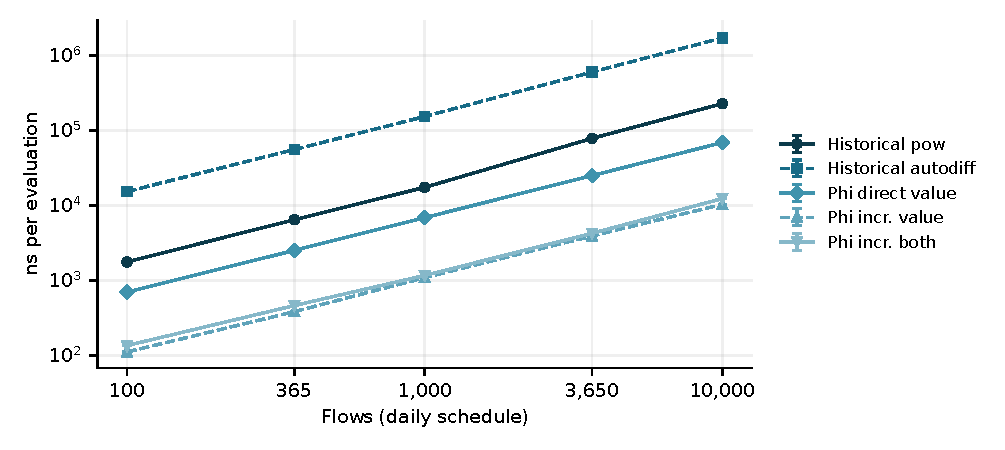
\includegraphics[width=0.78\linewidth]{generated/kernel.pdf}
\caption{Time for one NPV evaluation against the number of daily flows.}
\label{fig:kernel}
\end{figure}

\begin{center}\small
\resizebox{0.93\linewidth}{!}{\begin{tabular}{lrrrrr}
\toprule
Call & Daily (ns) & Weekly (ns) & Monthly (ns) & Irregular (ns) & Daily B/op \\
\midrule
Historical pow, value (boxed) & 4505 $\pm$ 18 & 4507 $\pm$ 17 & 4498 $\pm$ 14 & 4520 $\pm$ 29 & 0.0309 \\
Historical automatic differentiation (boxed) & 38820 $\pm$ 164 & 39086 $\pm$ 350 & 39090 $\pm$ 376 & 38953 $\pm$ 154 & 53712 \\
Pow, value (arrays) & 3940 $\pm$ 7 & 3940 $\pm$ 11 & 3946 $\pm$ 29 & 3934 $\pm$ 13 & 0.0270 \\
Pow, value and analytic derivative (arrays) & 4122 $\pm$ 31 & 4119 $\pm$ 17 & 4119 $\pm$ 30 & 4113 $\pm$ 20 & 32.03 \\
Phi direct, value & 1748 $\pm$ 6 & 1751 $\pm$ 10 & 1755 $\pm$ 7 & 1748 $\pm$ 7 & 0.0120 \\
Phi direct, value and derivative & 1864 $\pm$ 17 & 1858 $\pm$ 7 & 1866 $\pm$ 14 & 1860 $\pm$ 8 & 32.01 \\
Phi incremental, generic powers, value & 309.0 $\pm$ 5.0 & 726.1 $\pm$ 2.9 & 899.4 $\pm$ 45.5 & 4163 $\pm$ 16 & 0.0021 \\
Phi incremental, small powers, value & 278.4 $\pm$ 1.6 & 288.9 $\pm$ 0.9 & 917.2 $\pm$ 21.7 & 4221 $\pm$ 8 & 0.0019 \\
Phi incremental, small powers, value and derivative & 326.8 $\pm$ 2.2 & 335.4 $\pm$ 1.1 & 946.5 $\pm$ 17.7 & 4265 $\pm$ 16 & 32.00 \\
\bottomrule
\end{tabular}
}
\end{center}
\begin{center}\small
\begin{tabular}{lrrrr}
\toprule
Schedule & Pow/incr.\ value & Autodiff/incr.\ both & Generic/small-power incr. & Boxed/array pow \\
\midrule
Daily & 16.18 [16.03, 16.35] & 118.79 [117.48, 120.11] & 1.11 [1.09, 1.13] & 1.14 [1.14, 1.15] \\
Weekly & 15.60 [15.49, 15.71] & 116.54 [115.10, 117.98] & 2.51 [2.49, 2.53] & 1.14 [1.14, 1.15] \\
Monthly & 4.90 [4.78, 5.04] & 41.30 [40.15, 42.49] & 0.98 [0.91, 1.06] & 1.14 [1.13, 1.15] \\
Irregular & 1.07 [1.06, 1.08] & 9.13 [9.06, 9.20] & 0.99 [0.98, 0.99] & 1.15 [1.14, 1.16] \\
\bottomrule
\end{tabular}

\end{center}
Reading down the daily column:
\begin{itemize}\setlength{\itemsep}{0pt}
\item \textbf{Boxing} costs little on its own: arrays are $1.14\times$ faster for the same \code{Math.pow} loop.
\item \textbf{Automatic differentiation} is the expensive call: 38.8\,$\mu$s against 4.1\,$\mu$s for the analytic value and derivative on arrays, a factor of 9.4 (8.6 against one historical value), with \AllocAutodiff{} bytes allocated per evaluation.
\item \textbf{\code{exp} for \code{pow}}: the direct $\phi$ value is $2.25\times$ faster than the array \code{pow} value.
\item \textbf{The recurrence} is the largest single step: $5.7\times$ over direct exponentials on daily gaps, $6.3\times$ with the small-power cases.
\item \textbf{Small-power cases} matter where gaps fall in 2 to 7: $2.51\times$ on weekly gaps, $1.11\times$ on daily, nothing on monthly or irregular.
\end{itemize}
The recurrence depends on the schedule. On monthly gaps (28 to 31 days) each flow needs a square-and-multiply power and the advantage over \code{pow} falls to $4.9\times$. On irregular gaps the incremental value takes 4.2\,$\mu$s, which is $2.4\times$ \emph{slower} than direct exponentials (1.7\,$\mu$s) barely faster than the historical \code{pow} loop ($1.07\times$) and slower than \code{pow} on arrays. A likely cause is branch misprediction on exponents that change unpredictably from flow to flow; this was not profiled. The optimized solver always takes the incremental path, so this carries into its solve times (Section~\ref{sec:schedule}).

\subsection{Layer 2: preparation}
\begin{center}\small
\begin{tabular}{lrrrrr}
\toprule
Schedule & Three-pass ($\mu$s) & Digest ($\mu$s) & Ratio [envelope] & Three-pass B/op & Digest B/op \\
\midrule
Daily & 9.974 $\pm$ 0.032 & 3.706 $\pm$ 0.158 & 2.69 [2.57, 2.82] & 27568 & 5288 \\
Weekly & 9.811 $\pm$ 0.031 & 3.561 $\pm$ 0.104 & 2.76 [2.67, 2.85] & 27568 & 5288 \\
Monthly & 9.679 $\pm$ 0.024 & 3.607 $\pm$ 0.009 & 2.68 [2.67, 2.70] & 27568 & 5288 \\
Irregular & 11.42 $\pm$ 0.15 & 3.757 $\pm$ 0.075 & 3.04 [2.94, 3.14] & 27568 & 5288 \\
\bottomrule
\end{tabular}

\end{center}
The single-pass digest is 2.7 to 3.1 times faster than the three-pass boxed preparation and allocates a fifth of the memory. It also does more: the quantities for the existence analysis are gathered in the same pass.

\subsection{Layer 3: the ladder, class by class}\label{sec:classes}
\begin{figure}[t]
\centering
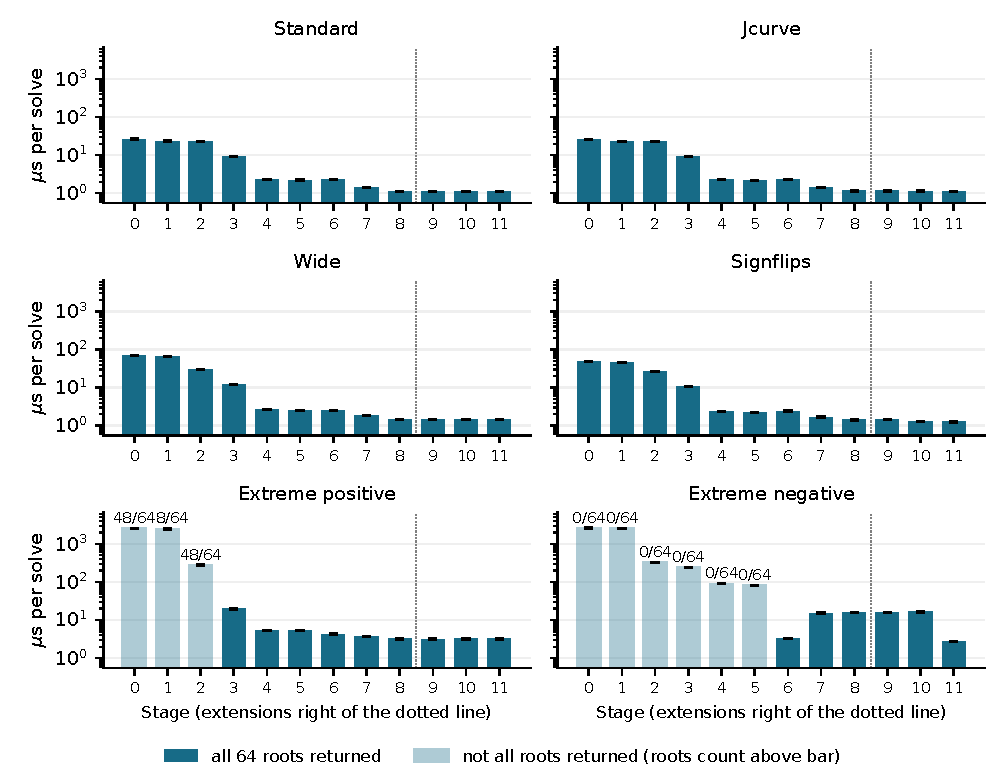
\includegraphics[width=0.86\linewidth]{generated/ladder.pdf}
\caption{Solve time per input at each stage, prepared input, 256 daily flows. Hatched bars mark stages that did not return all 64 roots, with the count above.}
\label{fig:ladder}
\end{figure}

\textbf{Standard.}
\begin{center}\small
\resizebox{\linewidth}{!}{\begin{tabular}{lrrrrrr}
\toprule
Stage & Time ($\mu$s) & Previous/current & L0/current & Roots/64 & Mean value evals & Mean deriv. evals \\
\midrule
L0 Historical & 24.84 $\pm$ 0.48 & --- & 1.00 & 64 & 5.5 & 0.0 \\
L1 Primitive arrays & 22.41 $\pm$ 0.35 & 1.11 [1.07, 1.15] & 1.11 [1.07, 1.15] & 64 & 5.5 & 0.0 \\
L2 Analytic derivative & 22.25 $\pm$ 0.10 & 1.01 [0.99, 1.03] & 1.12 [1.09, 1.14] & 64 & 5.5 & 0.0 \\
L3 Phi, direct exp & 8.905 $\pm$ 0.088 & 2.50 [2.46, 2.53] & 2.79 [2.71, 2.87] & 64 & 5.3 & 0.0 \\
L4 Incremental recurrence & 2.176 $\pm$ 0.010 & 4.09 [4.03, 4.15] & 11.41 [11.14, 11.69] & 64 & 5.5 & 0.0 \\
L5 Small-power cases & 2.105 $\pm$ 0.006 & 1.03 [1.03, 1.04] & 11.80 [11.54, 12.06] & 64 & 5.5 & 0.0 \\
L6 Analytic bounds & 2.136 $\pm$ 0.009 & 0.99 [0.98, 0.99] & 11.63 [11.36, 11.90] & 64 & 5.5 & 0.0 \\
L7 Newton first & 1.359 $\pm$ 0.005 & 1.57 [1.56, 1.58] & 18.27 [17.85, 18.69] & 64 & 0.0 & 2.8 \\
L8 Optimized & 1.097 $\pm$ 0.005 & 1.24 [1.23, 1.25] & 22.64 [22.09, 23.19] & 64 & 0.0 & 2.0 \\
\bottomrule
\end{tabular}
}
\end{center}
The historical solver stays on its Brent path for all 64 inputs: \MeanValuesStandardHistorical{} value evaluations and no derivative. Its time is the evaluation count times the kernel cost ($5.5\times4.5\,\mu$s). So L2 changes nothing here, because Newton never runs. The gains come from cheaper evaluations (L3 and L4, $2.5\times$ and $4.1\times$) and then from fewer of them: Newton first needs 2.8 combined evaluations instead of 5.5 values (L7, $1.57\times$), and the Pad\'e guess brings that to \MeanDerivativesStandardOptimized{} (L8, $1.24\times$). The analytic bracket alone (L6) costs about 1.5\%. At L8 two evaluations cost about 0.65\,$\mu$s of the 1.10\,$\mu$s; the remainder is moments, analysis and dispatch, so further kernel work would return little. The \emph{jcurve} class behaves the same at every stage and ends at $\SpeedupPreparedJcurve\times$.

\textbf{Wide.}
\begin{center}\small
\resizebox{\linewidth}{!}{\begin{tabular}{lrrrrrr}
\toprule
Stage & Time ($\mu$s) & Previous/current & L0/current & Roots/64 & Mean value evals & Mean deriv. evals \\
\midrule
L0 Historical & 65.58 $\pm$ 0.48 & --- & 1.00 & 64 & 6.0 & 1.0 \\
L1 Primitive arrays & 61.82 $\pm$ 0.28 & 1.06 [1.05, 1.07] & 1.06 [1.05, 1.07] & 64 & 6.0 & 1.0 \\
L2 Analytic derivative & 28.71 $\pm$ 0.26 & 2.15 [2.12, 2.18] & 2.28 [2.25, 2.32] & 64 & 6.0 & 1.0 \\
L3 Phi, direct exp & 11.55 $\pm$ 0.05 & 2.49 [2.45, 2.52] & 5.68 [5.61, 5.74] & 64 & 5.6 & 0.8 \\
L4 Incremental recurrence & 2.571 $\pm$ 0.008 & 4.49 [4.46, 4.52] & 25.51 [25.25, 25.77] & 64 & 5.9 & 0.8 \\
L5 Small-power cases & 2.393 $\pm$ 0.008 & 1.07 [1.07, 1.08] & 27.40 [27.11, 27.70] & 64 & 5.9 & 0.8 \\
L6 Analytic bounds & 2.422 $\pm$ 0.026 & 0.99 [0.97, 1.00] & 27.08 [26.60, 27.57] & 64 & 7.8 & 0.0 \\
L7 Newton first & 1.743 $\pm$ 0.012 & 1.39 [1.37, 1.41] & 37.62 [37.08, 38.16] & 64 & 0.0 & 3.9 \\
L8 Optimized & 1.390 $\pm$ 0.005 & 1.25 [1.24, 1.27] & 47.19 [46.66, 47.73] & 64 & 0.0 & 2.9 \\
\bottomrule
\end{tabular}
}
\end{center}
Nine of the 64 historical solves leave Brent and fall back to automatic-differentiation Newton. The mean is only one derivative evaluation per input, yet replacing it (L2) halves the time, because each such evaluation costs as much as 8.6 historical values. The overall speedup is $\SpeedupPreparedWide\times$. \emph{Signflips} is similar: seven historical solves use Newton, L2 gives $1.74\times$, and the total is $\SpeedupPreparedSignflips\times$.

\textbf{Extreme positive.}
\begin{center}\small
\resizebox{\linewidth}{!}{\begin{tabular}{lrrrrrr}
\toprule
Stage & Time ($\mu$s) & Previous/current & L0/current & Roots/64 & Mean value evals & Mean deriv. evals \\
\midrule
L0 Historical & 2521 $\pm$ 23 & --- & --- & 48 (failed 16) & 0.0 & 63.7 \\
L1 Primitive arrays & 2470 $\pm$ 23 & --- & --- & 48 (failed 16) & 0.0 & 63.7 \\
L2 Analytic derivative & 276.6 $\pm$ 3.1 & --- & --- & 48 (failed 16) & 0.0 & 63.5 \\
L3 Phi, direct exp & 19.53 $\pm$ 0.12 & --- & --- & 64 & 0.0 & 9.3 \\
L4 Incremental recurrence & 5.392 $\pm$ 0.048 & 3.62 [3.57, 3.68] & --- & 64 & 0.0 & 9.3 \\
L5 Small-power cases & 5.287 $\pm$ 0.040 & 1.02 [1.00, 1.04] & --- & 64 & 0.0 & 9.3 \\
L6 Analytic bounds & 4.277 $\pm$ 0.015 & 1.24 [1.22, 1.25] & --- & 64 & 13.3 & 0.0 \\
L7 Newton first & 3.629 $\pm$ 0.034 & 1.18 [1.16, 1.19] & --- & 64 & 0.0 & 8.4 \\
L8 Optimized & 3.177 $\pm$ 0.030 & 1.14 [1.12, 1.16] & --- & 64 & 0.0 & 7.2 \\
L9 Power table & 3.171 $\pm$ 0.019 & 1.00 [0.99, 1.02] & --- & 64 & 0.0 & 7.2 \\
L10 Ungated guess & 3.177 $\pm$ 0.027 & 1.00 [0.98, 1.01] & --- & 64 & 0.0 & 7.2 \\
L11 Log-form step & 3.180 $\pm$ 0.015 & 1.00 [0.99, 1.01] & --- & 64 & 0.0 & 7.2 \\
\bottomrule
\end{tabular}
}
\end{center}
The root lies above the rate bracket and the Dietz guess falls below it, so historical Brent is rejected before evaluating and every solve goes to Newton from 10\%. It takes 64 automatic-differentiation evaluations on average, converges for 48 inputs and fails for 16, at 2.5\,ms per input. The analytic derivative cuts that to 0.27\,ms with the same number of roots, though eight inputs swap between converging and failing. In $\phi$ (L3) the same Commons Newton converges for all 64 in 9.3 evaluations, plausibly because the function is better conditioned in the logarithmic coordinate. The optimized solver returns all 64 roots in 3.2\,$\mu$s. No ratio is printed against L0 because the outcomes differ.

\textbf{Extreme negative.}
\begin{center}\small
\resizebox{\linewidth}{!}{\begin{tabular}{lrrrrrr}
\toprule
Stage & Time ($\mu$s) & Previous/current & L0/current & Roots/64 & Mean value evals & Mean deriv. evals \\
\midrule
L0 Historical & 2619 $\pm$ 21 & --- & --- & 0 ($-$100\% fallback 64) & 0.1 & 200.0 \\
L1 Primitive arrays & 2521 $\pm$ 35 & --- & --- & 0 ($-$100\% fallback 64) & 0.1 & 200.0 \\
L2 Analytic derivative & 322.1 $\pm$ 0.9 & --- & --- & 0 ($-$100\% fallback 64) & 0.1 & 200.0 \\
L3 Phi, direct exp & 243.3 $\pm$ 1.9 & --- & --- & 0 (failed 64) & 0.1 & 200.0 \\
L4 Incremental recurrence & 90.03 $\pm$ 0.25 & --- & --- & 0 (failed 64) & 0.1 & 200.0 \\
L5 Small-power cases & 80.68 $\pm$ 0.50 & --- & --- & 0 (failed 64) & 0.1 & 200.0 \\
L6 Analytic bounds & 3.196 $\pm$ 0.011 & --- & --- & 64 & 10.5 & 0.0 \\
L7 Newton first & 15.17 $\pm$ 0.23 & 0.21 [0.21, 0.21] & --- & 64 & 11.8 & 30.0 \\
L8 Optimized & 15.95 $\pm$ 0.19 & 0.95 [0.93, 0.98] & --- & 64 & 13.3 & 30.0 \\
L9 Power table & 16.07 $\pm$ 0.14 & 0.99 [0.97, 1.01] & --- & 64 & 13.3 & 30.0 \\
L10 Ungated guess & 16.47 $\pm$ 0.46 & 0.98 [0.94, 1.01] & --- & 64 & 13.3 & 30.0 \\
L11 Log-form step & 2.694 $\pm$ 0.036 & 6.11 [5.86, 6.37] & --- & 64 & 0.0 & 5.1 \\
\bottomrule
\end{tabular}
}
\end{center}
Here the historical solver spends 200 automatic-differentiation evaluations and then returns its $-100\%$ fallback for every input: 2.6\,ms for no root. Stages L3 to L5 fail after 200 Newton evaluations, because the mapped bracket still excludes the root and the fallback step is gone. The analytic bracket (L6) is the change that matters: Brent finds all 64 roots in 10.5 evaluations and 3.2\,$\mu$s. Newton first then makes this class \emph{slower}. In all 64 cases Newton uses its 30 iterations without converging before Brent runs, and L7 and L8 take 15 to 16\,$\mu$s, five times L6. The cap of 30 bounds that cost; choosing Brent directly for a far-negative bound would remove it.

\textbf{Dominance.} No root exists. Stages L0 to L5 run 200 Newton evaluations and fail (2.7\,ms at L0, 0.2\,ms at L5). From L6 the analysis returns ``no solution'' with zero evaluations in 13\,ns.

\subsection{Schedule, size and seed}\label{sec:schedule}
\begin{center}\small
\begin{tabular}{lrrrr}
\toprule
Stage & Daily ($\mu$s) & Weekly ($\mu$s) & Monthly ($\mu$s) & Irregular ($\mu$s) \\
\midrule
L0 Historical & 24.84 $\pm$ 0.48 & 24.68 $\pm$ 0.11 & 24.77 $\pm$ 0.16 & 26.15 $\pm$ 0.20 \\
L1 Primitive arrays & 22.41 $\pm$ 0.35 & 22.33 $\pm$ 0.19 & 22.21 $\pm$ 0.11 & 23.58 $\pm$ 0.36 \\
L2 Analytic derivative & 22.25 $\pm$ 0.10 & 22.22 $\pm$ 0.11 & 22.26 $\pm$ 0.13 & 23.42 $\pm$ 0.09 \\
L3 Phi, direct exp & 8.905 $\pm$ 0.088 & 8.927 $\pm$ 0.075 & 8.883 $\pm$ 0.057 & 9.292 $\pm$ 0.075 \\
L4 Incremental recurrence & 2.176 $\pm$ 0.010 & 4.039 $\pm$ 0.014 & 5.579 $\pm$ 0.041 & 22.26 $\pm$ 0.13 \\
L5 Small-power cases & 2.105 $\pm$ 0.006 & 2.115 $\pm$ 0.005 & 5.577 $\pm$ 0.048 & 23.05 $\pm$ 0.19 \\
L6 Analytic bounds & 2.136 $\pm$ 0.009 & 2.147 $\pm$ 0.009 & 5.542 $\pm$ 0.089 & 23.31 $\pm$ 0.23 \\
L7 Newton first & 1.359 $\pm$ 0.005 & 1.394 $\pm$ 0.010 & 3.412 $\pm$ 0.032 & 12.53 $\pm$ 0.13 \\
L8 Optimized & 1.097 $\pm$ 0.005 & 1.083 $\pm$ 0.003 & 2.607 $\pm$ 0.020 & 9.757 $\pm$ 0.100 \\
\bottomrule
\end{tabular}

\end{center}
The standard class on four schedules shows which stages depend on the schedule. Everything up to L3 does not: \code{pow} and \code{exp} do not care about gaps. The recurrence (L4) gains $4.1\times$ on daily gaps, $2.2\times$ on weekly, $1.6\times$ on monthly, and on irregular gaps it \emph{loses} a factor of 2.4, returning to the cost of L1. Small-power cases (L5) recover the weekly schedule. The overall speedup is therefore $22.8\times$ weekly, $9.5\times$ monthly and $2.7\times$ irregular (headline table). An optimized solver that chose the direct path for irregular schedules would be faster there.

Two further seeds give $22.5\times$ and $22.9\times$ for the standard class. With 16 flows the speedup is $10.5\times$, since fixed work dominates a 0.16\,$\mu$s solve; with 4{,}096 flows it is $25.9\times$.

\subsection{Preparation included}
With dated input the standard speedup is $\SpeedupDatedStandard\times$ rather than $\SpeedupPreparedStandard\times$. The difference between dated and prepared solves is 9.8 of 34.6\,$\mu$s for the historical solver and 3.9 of 5.0\,$\mu$s for the optimized one: after the search has been reduced to about 1\,$\mu$s, the digest is the larger part of the work, and it is the next thing to optimize for callers that solve each input once.

\subsection{Accuracy}\label{sec:accuracy}
\begin{center}\small
\resizebox{0.9\linewidth}{!}{\begin{tabular}{lrrrrrrrr}
\toprule
Class & Agree & Disagree & Only H & Only L8 & H $-$100\% fallback & Neither & Max residual H & Max residual L8 \\
\midrule
Standard & 64 & 0 & 0 & 0 & 0 & 0 & $4.4\times10^{-7}$ & $7.4\times10^{-14}$ \\
Wide & 64 & 0 & 0 & 0 & 0 & 0 & $2.1\times10^{-6}$ & $6.5\times10^{-14}$ \\
Jcurve & 64 & 0 & 0 & 0 & 0 & 0 & $4.8\times10^{-7}$ & $6.1\times10^{-14}$ \\
Signflips & 63 & 1 & 0 & 0 & 0 & 0 & $1.9\times10^{-7}$ & $1.1\times10^{-10}$ \\
Extreme positive & 48 & 0 & 0 & 16 & 0 & 0 & $5.2\times10^{-16}$ & $9.7\times10^{-16}$ \\
Extreme negative & 0 & 0 & 0 & 0 & 64 & 0 & --- & $6.4\times10^{-7}$ \\
Dominance & 0 & 0 & 0 & 0 & 0 & 64 & --- & --- \\
\bottomrule
\end{tabular}
}
\end{center}
The table compares the two endpoints on the 64 inputs of each class (256 daily flows, seed 42); roots agree when the rates differ by at most $10^{-5}$ (relative to the rate above 1, and in $\phi$ when $|\phi|>5$). On the standard, wide and jcurve classes all roots agree, as do the 48 joint roots of the extreme-positive class. Historical residuals reach $10^{-7}$ to $10^{-6}$ because Brent results are rounded down to six decimals; the optimized Newton result is not rounded and its residuals stay below $10^{-13}$. The optimized residual on the extreme-negative class is larger because those roots come from Brent.

One signflips input disagrees. The historical solver returns $-5.8\%$, the constructed root. The optimized solver is directed to the positive side, where a root is guaranteed, and the diagnostics record five Newton iterations followed by Brent. Replaying the case shows Newton converging to the negative root, which the direction gate rejects. Brent then returns a second, remote root at a rate near $3\times10^{107}$ with residual $1.1\times10^{-10}$. Both are roots of Equation~\eqref{eq:rate}. The analysis guarantees existence, not uniqueness or economic relevance.

\section{Limitations and disclosures}
\begin{itemize}\setlength{\itemsep}{1pt}
\item \textbf{Evidence base.} Synthetic inputs, one machine, one JDK. Both solvers are reconstructions of documented designs. The reconstruction builds no diagnostic messages on failure, so historical times on failing classes are, if anything, understated.
\item \textbf{Bundled changes.} L3, L4, L6 and L7 each carry the side effects listed in Section~\ref{sec:ladder}. The step from L3 to L4 on negative roots, and from L6 to L7, should be read with that in mind.
\item \textbf{Schedule dependence.} The recurrence is slower than direct exponentials on irregular gaps, and the optimized solver does not switch paths (Sections~\ref{sec:kernel} and~\ref{sec:schedule}).
\item \textbf{Newton first on far-negative roots.} It costs 30 wasted iterations per solve (Section~\ref{sec:classes}).
\item \textbf{Multiple roots.} With several roots the two solvers can return different ones, including roots far outside any plausible range (Section~\ref{sec:accuracy}). At L6, five signflips solves return a valid, strongly negative $\phi$ whose rate rounds to $-100\%$ in double precision; they are counted as roots.
\item \textbf{Brent's function-value threshold.} Brent is constructed with a coordinate tolerance only, which leaves the Commons default absolute function threshold of $10^{-15}$. With extremely small amounts it can accept an unrefined point. A disabled test records this for stages L3 to L6.
\item \textbf{Unguarded Newton before L7.} The Commons Newton used at L0 to L6 accepts a vanishing step as convergence and can report a spurious root. This occurred on one no-root input in the stress suite (at L4 and L5) and on none of the \DiagnosticRows{} diagnostic rows.
\item \textbf{Not timed.} The terminal cases are decided before any search and are not benchmarked. Same-day opposing flows give an infinite analytic bound and are not in the corpus.
\item \textbf{Kernel detail.} Calls returning value and derivative allocate a 32-byte result record in the kernel benchmark; that cost is included.
\end{itemize}

\section{Conclusions}
\begin{enumerate}\setlength{\itemsep}{1pt}
\item \textbf{Evaluation cost dominates the common case.} On standard flows the historical solver never computes a derivative, so its cost is five or six \code{Math.pow} sweeps. Replacing \code{pow} with \code{exp} and then with a recurrence accounts for a factor of 10 of the 23; Newton first with a Pad\'e guess supplies the remaining factor of two by cutting evaluations from 5.5 to 2.0.
\item \textbf{Automatic differentiation dominates the uncommon case.} One such evaluation costs nine value evaluations and allocates 54\,kB. Wherever the historical solver leaves Brent, it pays for this up to 200 times.
\item \textbf{The analytic bracket changes outcomes, not speed.} It does nothing for standard inputs. Below the historical bracket it turns failures (80\,$\mu$s at L5, 2.6\,ms at L0) into roots in 3\,$\mu$s, and where no root exists it replaces 200 evaluations with a 13\,ns proof.
\item \textbf{Two changes cost time on some inputs.} The recurrence loses to direct exponentials on irregular gaps, and Newton first loses to Brent on far-negative roots. Both are measured here and both have a simple remedy: choose the evaluation path by schedule and the first method by bound.
\item \textbf{End to end, preparation is next.} Once the search takes 1\,$\mu$s, the 3.6 to 3.9\,$\mu$s digest limits the dated speedup to about 7.
\end{enumerate}

\section*{Reproducibility}
\code{./mvnw -B clean verify} builds and tests; \code{scripts/study.sh full} runs the study (about 95 minutes); \code{scripts/verify\_evidence.py} and \code{scripts/analyze.py} check the evidence and regenerate every table, figure and number above from the raw JMH output and diagnostics retained under \code{results/}.

\bibliographystyle{plain}
\bibliography{references}
\end{document}
